%!TEX program = xelatex
\PassOptionsToPackage{quiet}{xeCJK}
\documentclass[notes=beamer]{ctexbeamer}

\usepackage[bluetheme]{ustcbeamer}
\usepackage[export]{adjustbox}
\usepackage{subfigure}
\usepackage{float}
\usepackage{cite}
\usepackage{threeparttable}
\usepackage{booktabs}
\usepackage{multirow}

% Removes icon in bibliography
\setbeamertemplate{bibliography item}[text]
\setbeamertemplate{caption}{\raggedright\insertcaption\par}
                          %%% ustcbeamer说明 %%%%
%% 宏包使用了TikZ代码形式的背景文件(在子文件夹theme中),默认选项"bluetheme",是科大校徽的蓝色;此外ustcbeamer还内置了红色和黑色主题"redtheme","blacktheme"。

                        %%% 自定义你的主题颜色 %%%
%% 一旦使用了下述命令就会覆盖ustcbeamer的内置颜色选项,你可以设置自己喜欢的RGB色值:
% \definecolor{themecolor}{RGB}{0,150,0} % 这是绿色主题
% \definecolor{themecolor}{RGB}{0,150,150} % 青色主题,也蛮好看的

%% 注意小写rgb和大写RGB表示的色值相差255倍,即RGB{255,255,255}=rgb{1,1,1};
% \definecolor{themecolor}{rgb}{0,0.5,0.3} % 深绿色主题

%% 建议自定义的主题颜色选择偏深色
%%%%%%%%%%%%%%%%%%%%%%%%%%%%%%%%%%%%%%%%%%%%%%%%%%%%%%%%%%%%%%%%%%%%%%


\title[图神经网络计算图耗时预测]{
  基于图神经网络的深度学习计算图耗时预测
}
\author[吴钰同]{答辩人:吴钰同\inst{1}\\[1ex]  {指导教师:张昱\inst{1} 张曦珊\inst{2}}}
\institute[USTC]{
\inst{1} 中国科学技术大学,计算机科学与技术学院 \and  \inst{2} 中国科学院,计算技术研究所
}
\date{\today}
\begin{document}
%\section<⟨mode specification⟩>[⟨short section name⟩]{⟨section name⟩}
%小于等于六个标题为恰当的标题

%--------------------
%标题页
%--------------------
\maketitleframe
\note{各位老师好,我是吴钰同,我的毕设题目是《基于图神经网络的深度学习计算图耗时预测》。}

%--------------------
%目录页
%--------------------
%beamer 101
\begin{frame}%
	\frametitle{大纲}%
	\tableofcontents[hideallsubsections]%仅显示节
	%\tableofcontents%显示所节和子节
  \note{
    我的答辩将分为以下五部分。首先我来介绍一下深度学习编译技术和计算图耗时预测任务的相关背景。
  }
\end{frame}%
%--------------------
%节目录页
%--------------------
\AtBeginSection[]{
\setbeamertemplate{footline}[footlineoff]%取消页脚
  \begin{frame}%
    \frametitle{大纲}
	%\tableofcontents[currentsection,subsectionstyle=show/hide/hide]%高亮当前节,不显示子节
    \tableofcontents[currentsection,subsectionstyle=show/show/hide]%show,shaded,hide
  \end{frame}
\setbeamertemplate{footline}[footlineon]%添加页脚
}
%--------------------
%子节目录页
%--------------------
\AtBeginSubsection[]{
\setbeamertemplate{footline}[footlineoff]%取消页脚
  \begin{frame}%
    \frametitle{大纲}
	%\tableofcontents[currentsection,subsectionstyle=show/hide/hide]%高亮当前节,不显示子节
    \tableofcontents[currentsection,subsectionstyle=show/shaded/hide]%show,shaded,hide
  \end{frame}
\setbeamertemplate{footline}[footlineon]%添加页脚
}

\section{研究背景}

\begin{frame}[c]
  \frametitle{深度学习编译技术}
  深度学习编译器:用于将\textbf{深度神经网络程序}高效地部署到具有不同\textbf{体系结构特点}的处理器上。
  \begin{figure}[h]
    \centering
    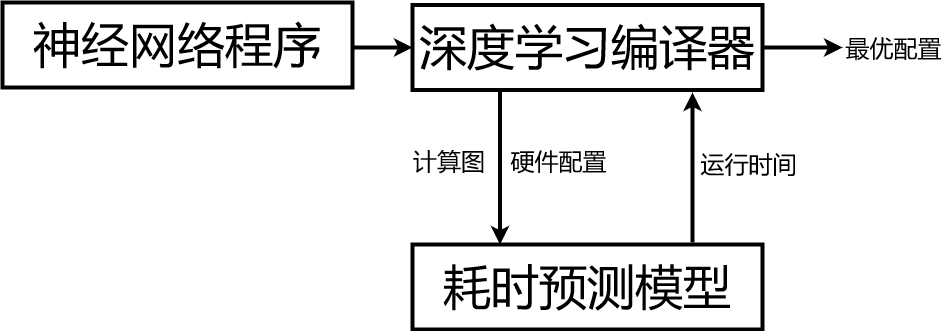
\includegraphics[width=0.9\textwidth]{figures/compilerOverview.png}
    \caption{深度学习编译器示意图}
  \end{figure}
  \note{
    深度学习编译器用于将神经网络程序高效的部署到具有不同结构特点的处理器上。
    为了确定最短运行时间所对应的编译配置,深度学习编译器通过耗时预测模型估计在特定硬件配置下程序的运行时间。
  }
\end{frame}

\begin{frame}[c]
  \frametitle{计算图耗时预测任务}
  \begin{figure}
    \centering
    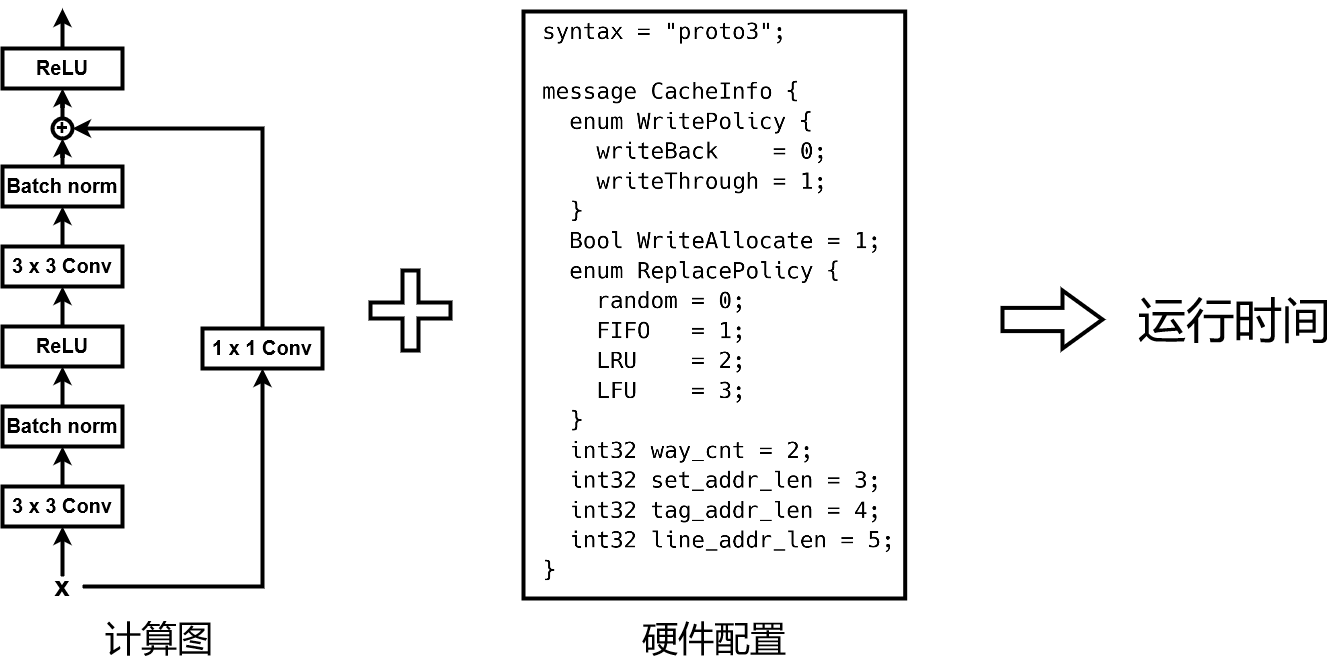
\includegraphics[width=1\textwidth]{figures/cg.png}
    \caption{计算图耗时预测任务示意图}
  \end{figure}
  \note{
    计算图耗时预测模型的输入是计算图和编译配置,输出是估计的程序运行时间。计算图就是以图的形式描述的神经网络,其中结点代表算子,边代表数据。编译配置就是具体的硬件信息。
  }
\end{frame}

\section{相关工作}

\begin{frame}
  \frametitle{传统模型和 LSTM 模型}
  \begin{itemize}
  \item 传统耗时预测方法使用\textbf{经验公式}\footnote[1]{Paleo, ICLR17}预测计算图的执行时间,例如:
  \footnote[2]{其中 $\mathcal{R}(u)$ 表示 $v$ 从前驱结点 $u$ 获取数据所需的时间。
  $\mathcal{C}(f_v,d_v)$ 表示 $v$ 对应算子 $f_v$ 在给定硬件 $d_v$ 上计算所需时间,
  $\mathcal{W}(f_v,d_v)$ 表示把运算结果写入 $d_v$ 的存储器所需要的时间。}
  $$
    T(v) = \sum \limits_{(u, v) \in \mathcal{E}}
    \mathcal{R} (u) + \mathcal{C}(f_v,d_v) + \mathcal{W}(f_v,d_v)
  $$
    \item 假设处理器按照\textbf{拓扑序}依次处理计算图的每个结点,并把这些结点当作\textbf{时间序列},则可以使用基于 LSTM 的 DAG-RNN 模型\footnote[3]{Ithemal, PMLR19}预测时间。
  \end{itemize}
  \note{
    下面来介绍一些现有的耗时预测模型。传统的耗时预测方法是使用经验公式估计程序执行时间,有准确率低和可扩展性差的特点。
    如果我们将计算图的结点视作时间序列,则可以使用 LSTM 模型进行耗时预测。
  }
\end{frame}

\begin{frame}[b]
  \frametitle{用图神经网络进行计算图耗时预测}
  谷歌提出使用\textbf{图神经网络}模型进行计算图耗时预测。
  \begin{figure}[t]
    \centering
    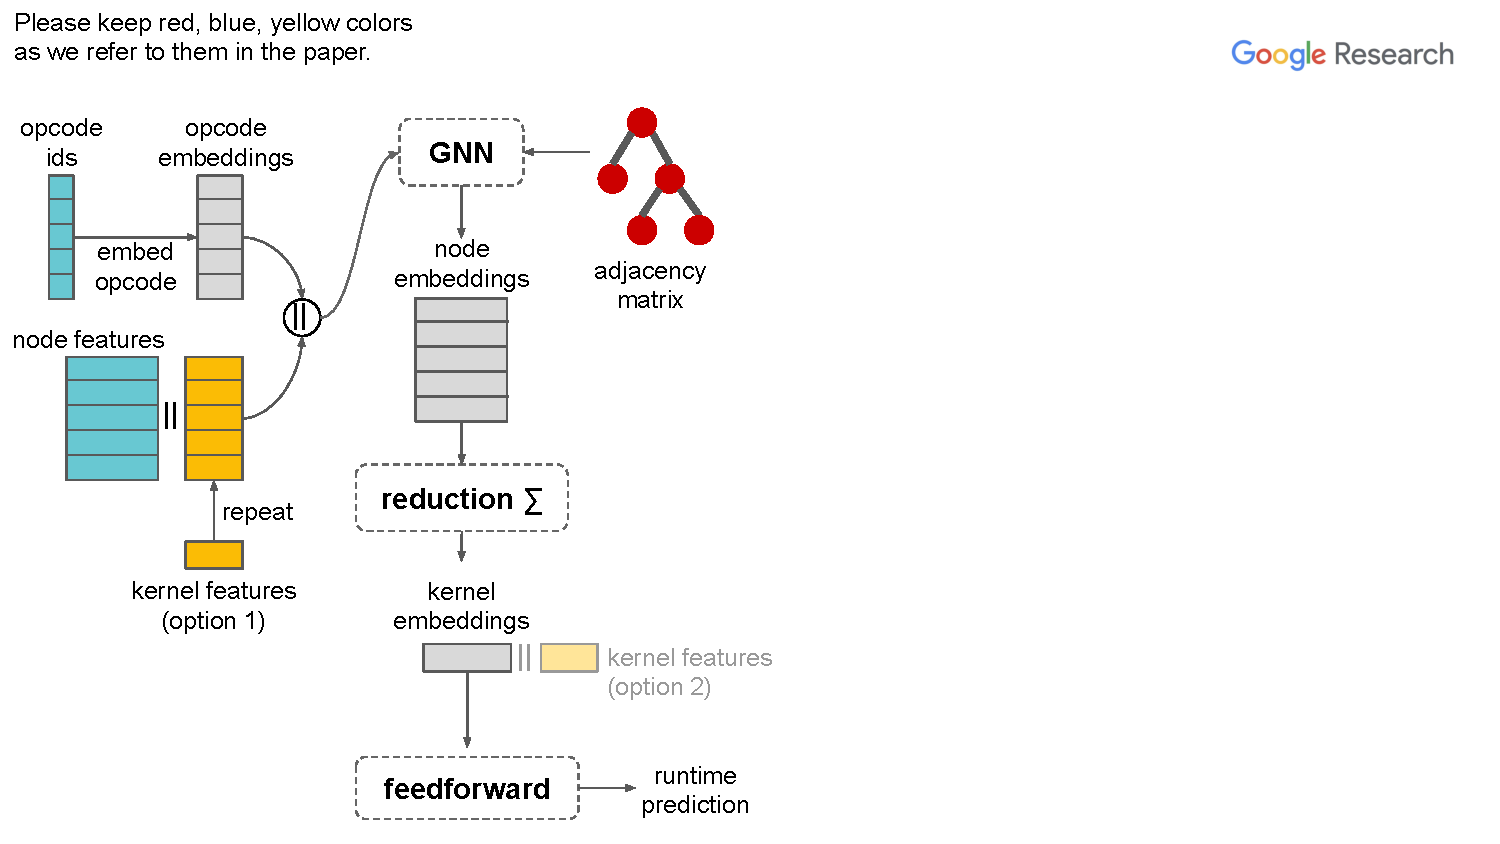
\includegraphics[width=0.5\textwidth,trim={0cm .42cm 12cm 1.2cm},clip]{figures/model3.pdf}
    \caption{图神经网络计算图耗时预测模型示意图 \footnote[1]{Google, MLSys21}}
  \label{fig:overview}
  \end{figure}
  \note{
    谷歌在 MLSys21 的一篇论文中提到可以使用图神经网络进行计算图耗时预测。\\
    我参考该论文复现了基于图神经网络的计算图耗时预测模型,并进行了一定的改进。\\
    以下就是我的具体方案。
  }
\end{frame}

\section{方案介绍}

\begin{frame}[b]
  \frametitle{图神经网络介绍}
  图神经网络:能够处理\textbf{图数据结构}的神经网络。通过聚合邻居结点和边的特征来利用图的拓扑结构信息。
  \begin{figure}[h]
    \centering
    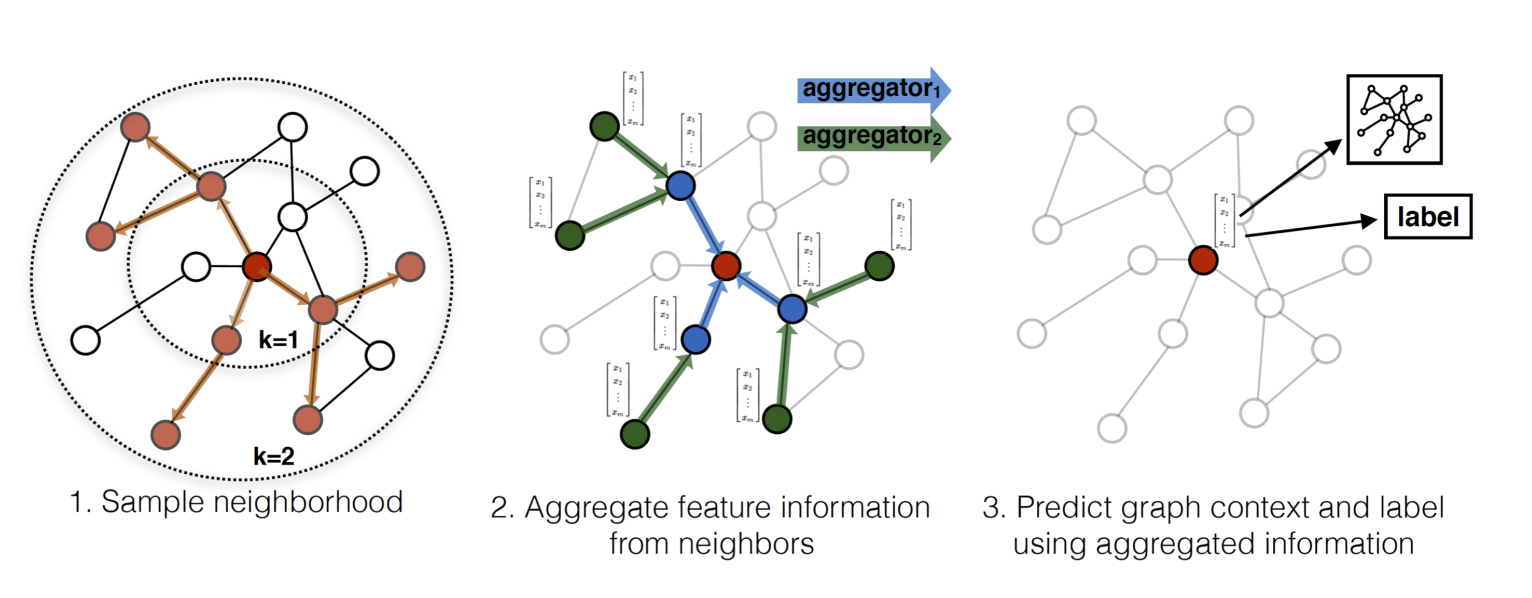
\includegraphics[width=1\textwidth]{figures/GNN.png}
    \caption{图神经网络示意图 \footnote[1]{GraphSAGE, NIPS17}}
  \end{figure}
  \note{
    图神经网络是一种专门用于处理图数据的神经网络。相比于传统的神经网络,图神经网络可以使图数据的特征信息在邻居结点之间传递和聚合,从而充分利用图的拓扑结构,而不是像传统的神经网络模型一样将图数据视作孤立的结点和边。
  }
\end{frame}

\begin{frame}[b]
  \frametitle{耗时预测流程}
  我使用的耗时预测方法包括以下三个部分:
  \begin{itemize}
    \item 提取 MLIR 和硬件配置的\textbf{特征}以及计算图的\textbf{邻接关系}
    \item 将相关特征进行\textbf{编码},生成特征向量
    \item 将特征向量和计算图的邻接关系输入\textbf{耗时预测模型},得到预测时间
  \end{itemize}
  \begin{figure}[h]
    \centering
    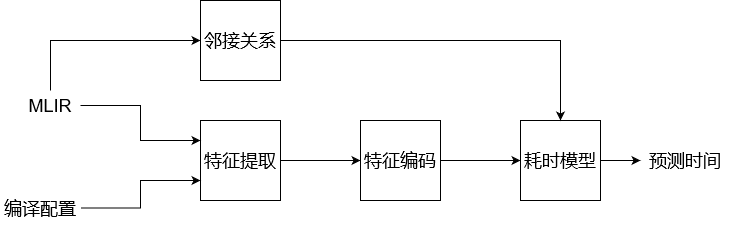
\includegraphics[width=0.9\textwidth]{figures/model_overall.png}
    \caption{耗时预测流程图}
  \end{figure}
  \note{
    我使用的耗时预测方法的主要流程如下:首先从深度学习编译器的中间表示 MLIR
    和硬件配置中提取特征和邻接关系,然后对其进行编码,最后使用图神经网络模型进行耗时预测。
  }
\end{frame}

\begin{frame}[b]
  \frametitle{图数据结构}
  从 MLIR 中提取\textbf{计算图特征}和\textbf{结构}信息:
  \begin{figure}[h]
    \centering
    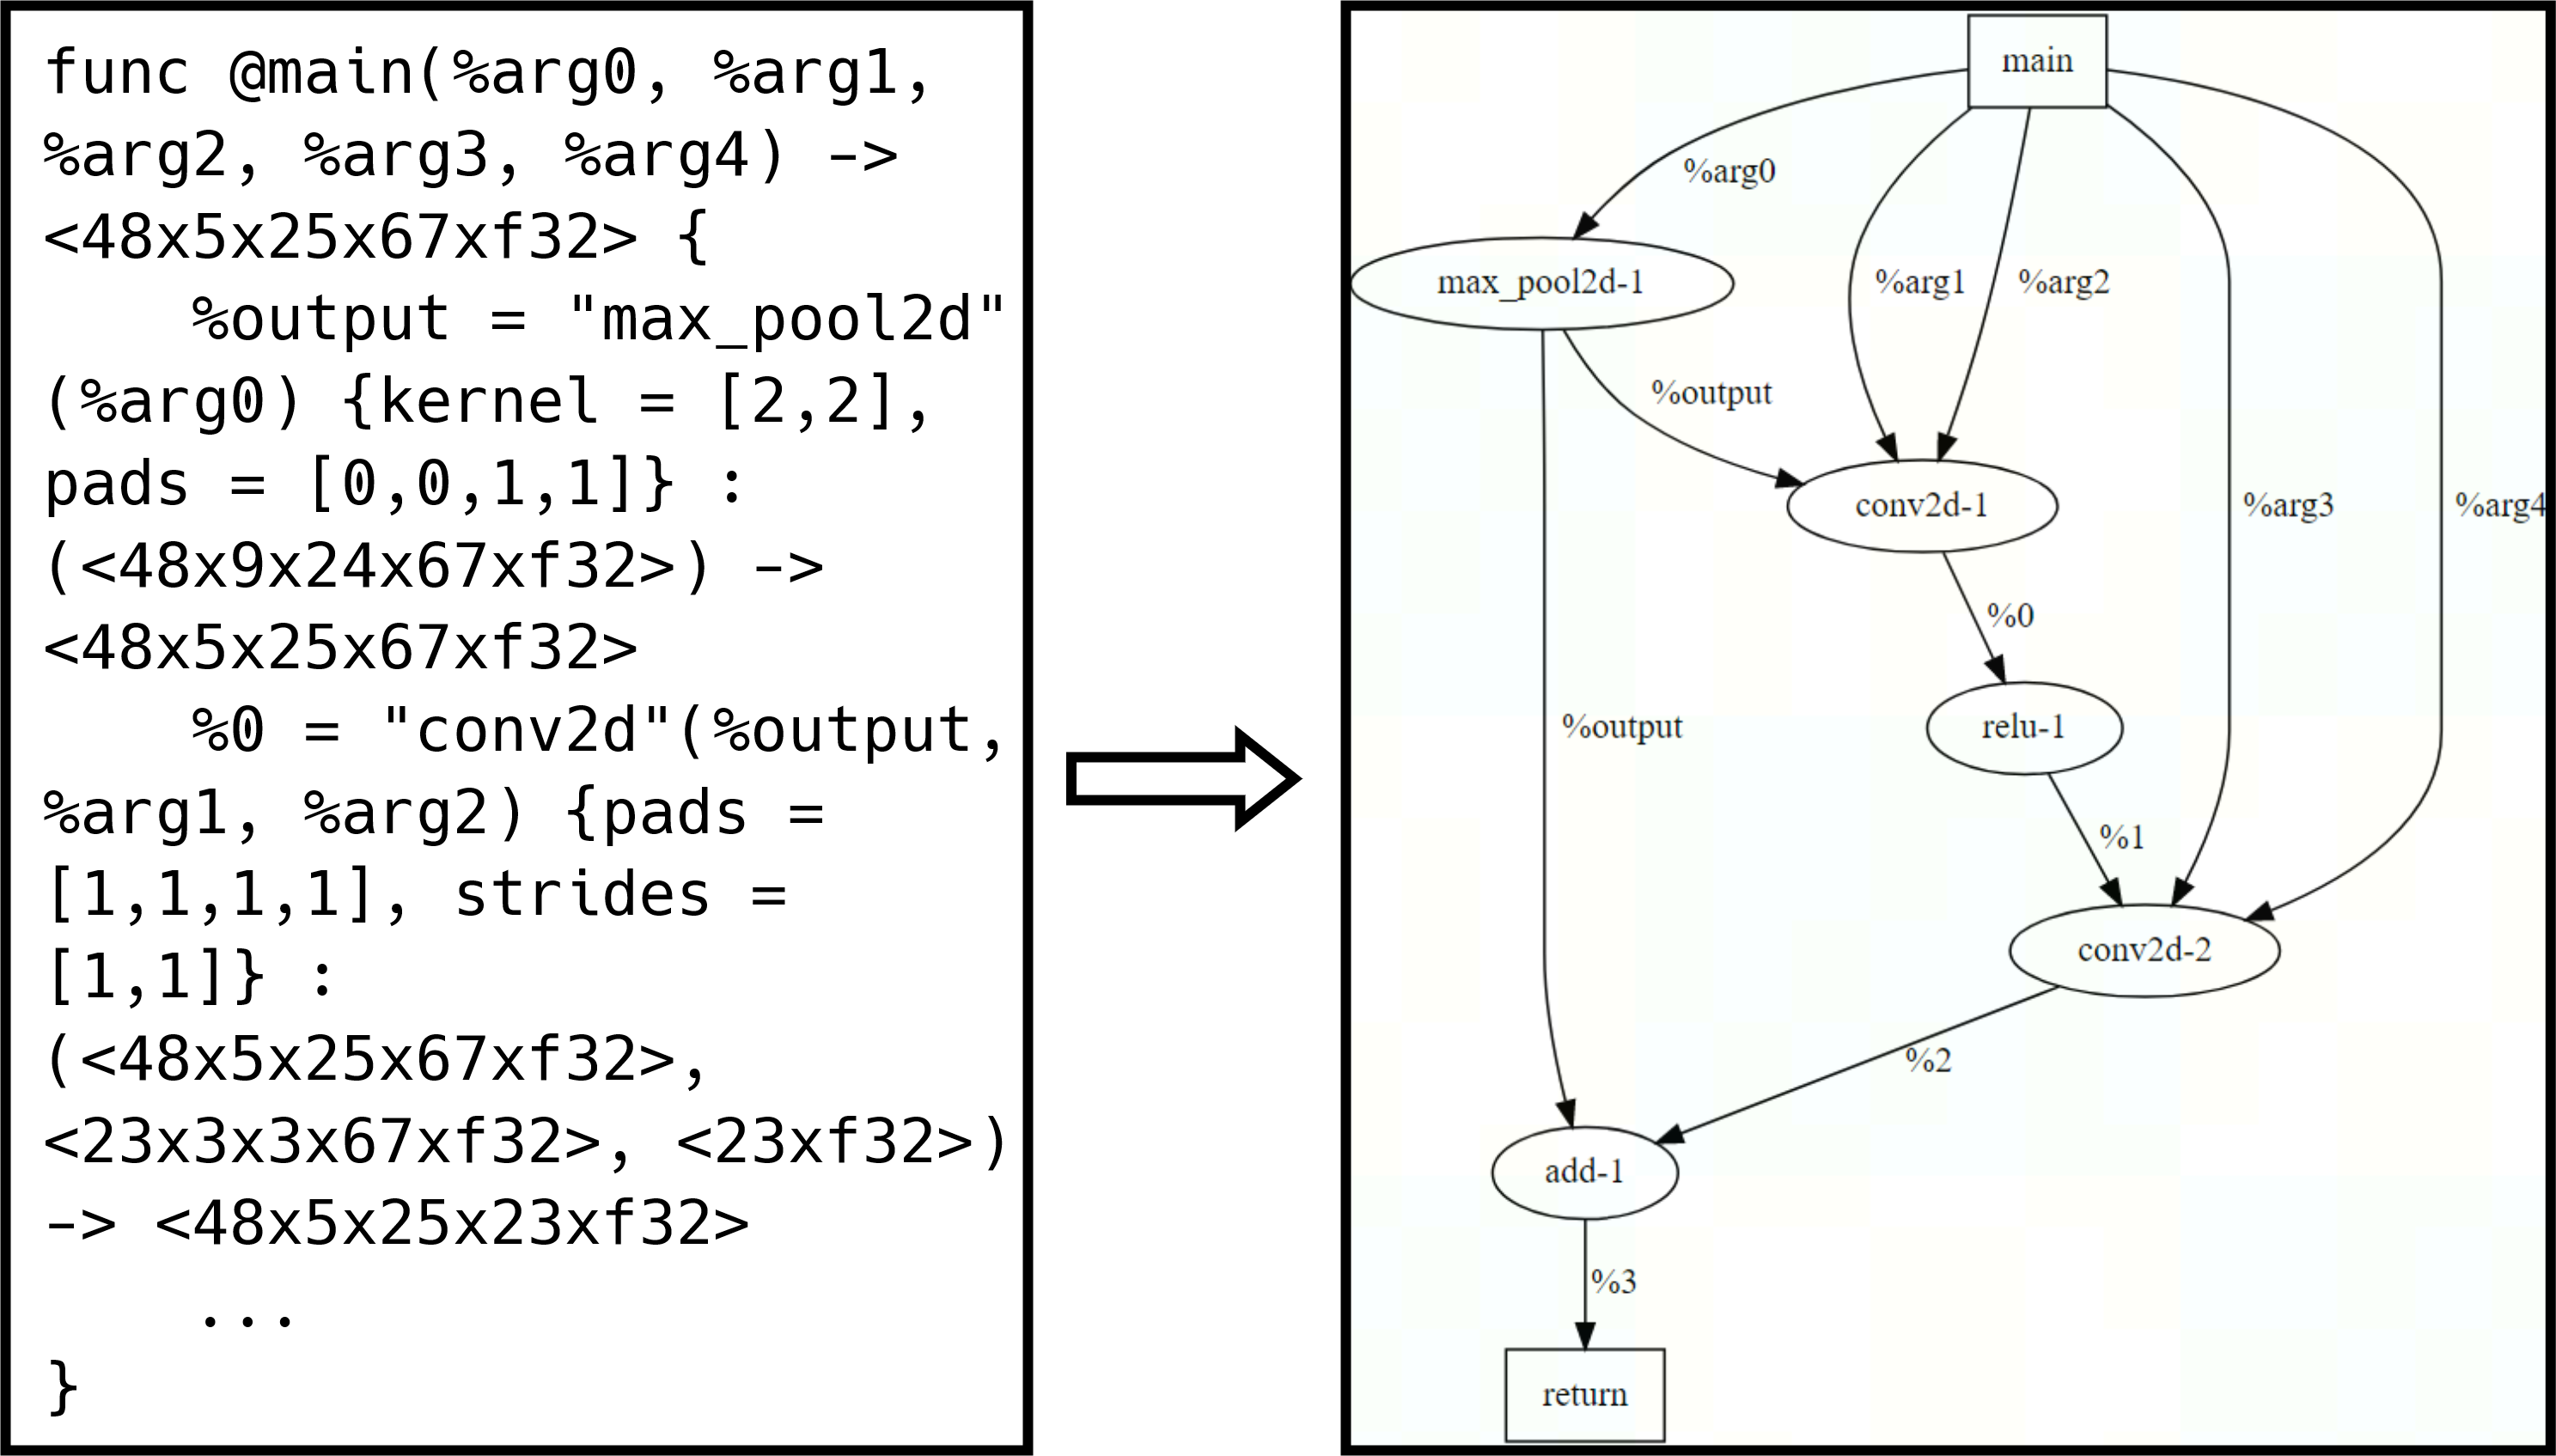
\includegraphics[width=1\textwidth]{figures/encode.png}
  \end{figure}
  \note{
    具体来说,我首先从深度学习编译器的中间表示 MLIR 中提取计算图的信息,以卷积算子为例,我们需要提取卷积核的维度和精度,填充的元素个数和步长,以及它与哪些结点邻接等信息。
  }
\end{frame}

\begin{frame}[b]
  \frametitle{特征编码}
  对计算图和编译配置的特征进行\textbf{编码}:
  \begin{figure}[h]
    \centering
    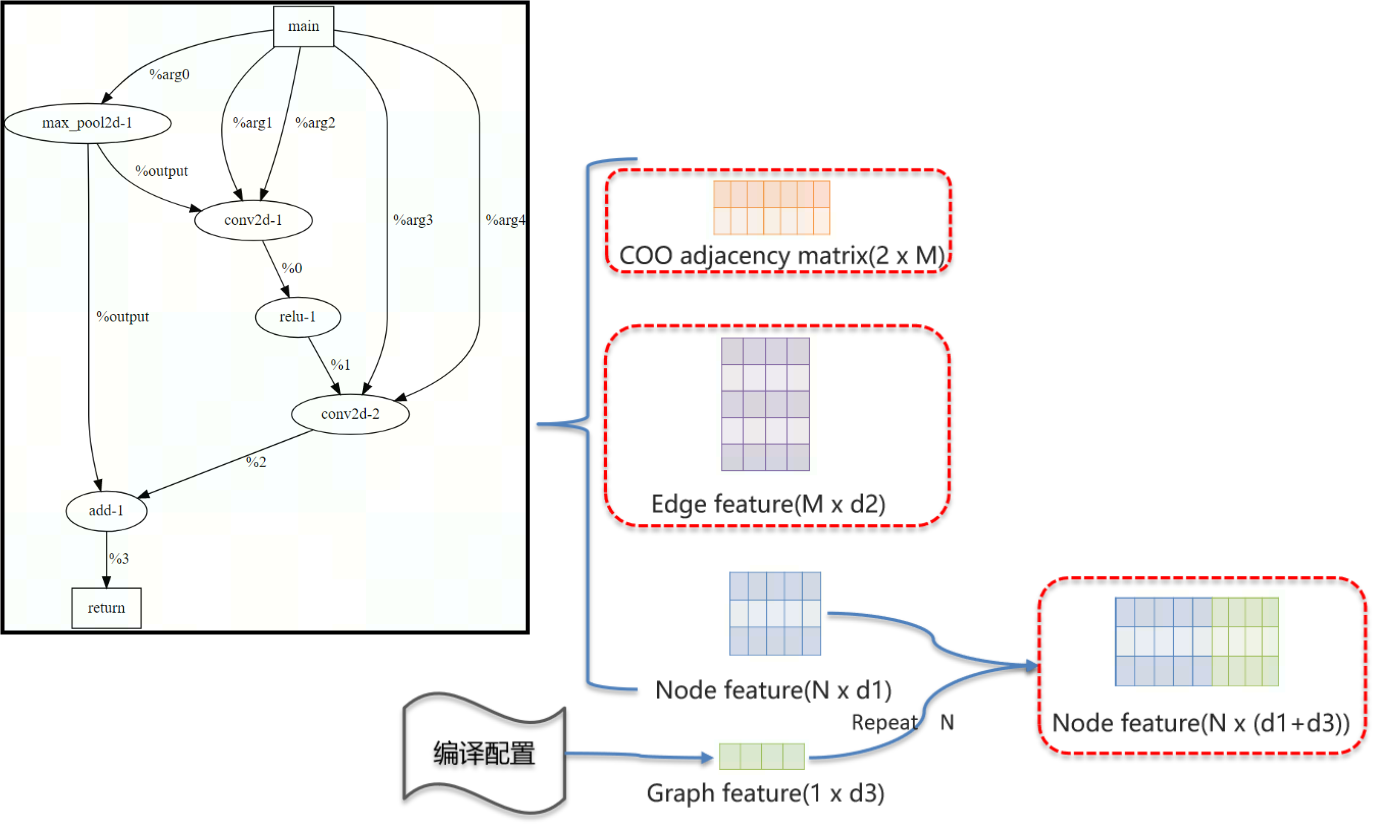
\includegraphics[width=0.95\textwidth]{figures/encode2.png}
  \end{figure}
  \note{
    然后,我们对从计算图和编译配置中的特征信息进行编码。计算图的特征信息包括用于表示邻接关系的邻接矩阵、作为结点特征的算子属性和作为边特征的张量属性。
    对于编译配置,由于整张计算图需要在同样的硬件配置下进行编译,所以我们将编译配置属性作为整个图数据的特征,将其拼接到每一个结点的特征向量的后面。\\
    最后我们得到一系列的结点特征向量和边特征向量,将它们作为耗时预测模型的输入。
  }
\end{frame}

\begin{frame}[b]
  \frametitle{模型设计}
  将特征向量和图结构信息输入\textbf{图神经网络模型},得到预测时间:
  \begin{figure}
    \centering
    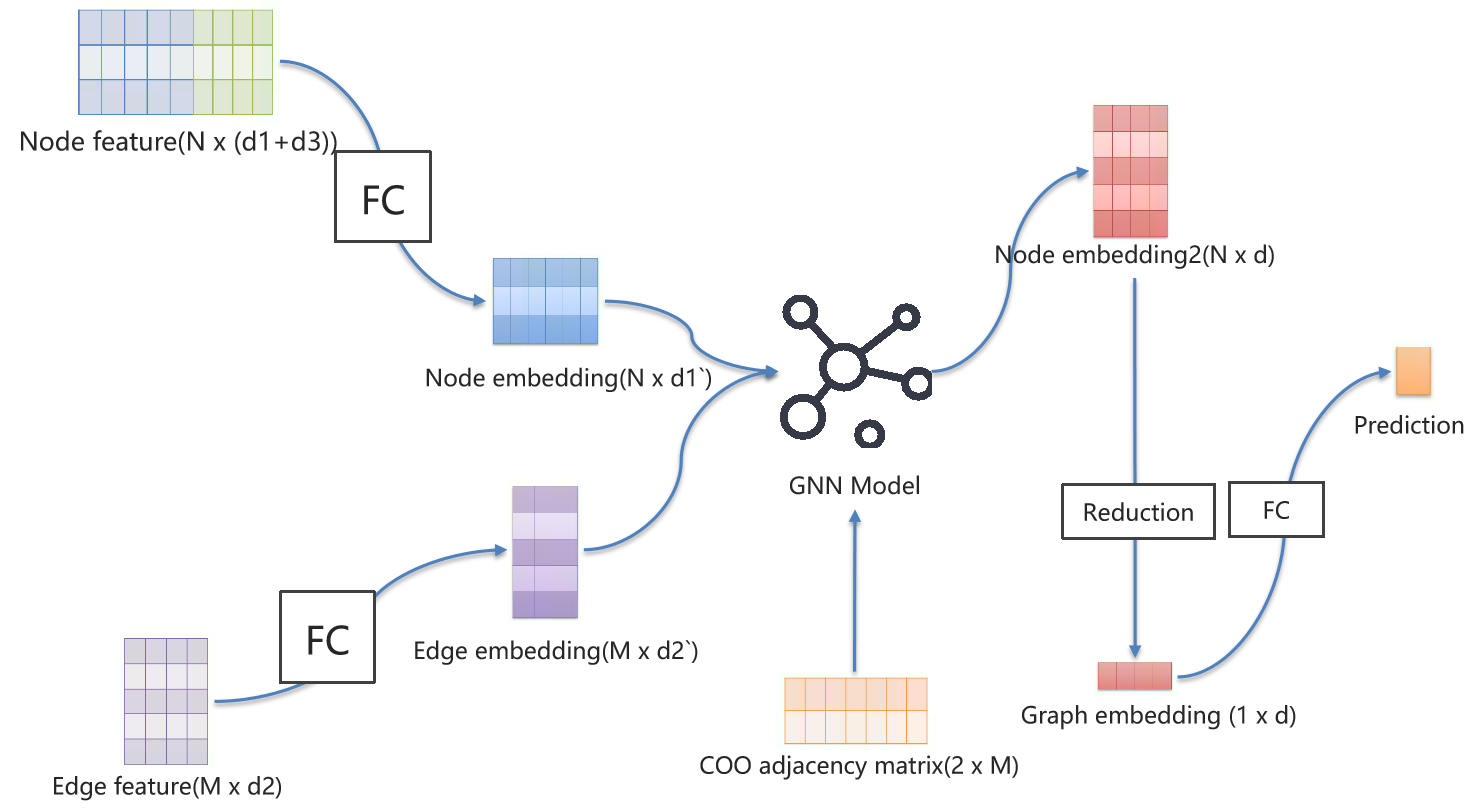
\includegraphics[width=1\textwidth]{figures/model.png}
  \end{figure}
  \note{
    我们使用的模型结构如下:为了学习特征之间的相似关系,同时降低特征空间的维度,我们先将结点和边的特征向量通过传统的全连接神经网络嵌入到低维向量空间中。\\
    随后,使用图神经网络聚合结点和边的特征得到新的嵌入向量,最后所有结点向量逐元素相加得到整个图的特征向量,将其通过一个全连接层得到预测时间。
  }
\end{frame}

\begin{frame}
  \frametitle{损失函数}
  \textbf{损失函数}在神经网络中用于刻画预测值与真实值的偏差,从而使用\textbf{反向传播}技术调整各层网络参数。
  我所使用的损失函数如下:
  \begin{itemize}
    \item   
    \textbf{平均平方误差}(mean squared error, MSE)是最常用的损失函数,其计算公式如下:
    \begin{align*}
      \mathbf{MSE} = \frac 1n \sum \limits_{i=1}^n (Y_i - \hat{Y}_i)^2
    \end{align*}
    \item
    \textbf{平均绝对误差}(mean absolute error, MAE)采用绝对值来代替平方运算,减少了\textbf{极端数据}对误差的影响:
    \begin{align*}
      \mathbf{MAE} = \frac 1n \sum \limits_{i=1}^n |Y_i - \hat{Y}_i|
    \end{align*}
  \end{itemize}
  \note{
     为了在训练中使用反向传播,我尝试了 MSE 和 MAE 两种损失函数。由于我使用的数据集存在一些
     极端数据,故 MAE 的实际效果更好。
  }
\end{frame}

\begin{frame}
  \frametitle{评价指标}
  评价指标用于衡量模型的\textbf{泛化性},即模型在训练集之外的\textbf{验证集和测试集}上的预测效果,我主要使用的评价指标如下:
  \begin{itemize}
    \item 
    \textbf{肯德尔秩相关系数}(Kendall rank correlation coefficient)是用于衡量两个\textbf{排序}\textbf{相似程度}的指标,其取值在 -1 和 1 之间,越接近 1 表示越相似。

    若两个排序分别为 $x = (x_1,x_2, ..., x_n)$ 和 $y = (y_1,y_2, ..., y_n)$,则 $x$ 和 $y$ 之间的肯德尔秩相关系数计算如下:
    \footnote{其中,$n_c$ 为所有满足 $i < j$ 的 $(x_i, x_j)$ 与 $(y_i,y_j)$ 中大小关系一致的 $(i,j)$ 对的个数,$n_d$ 为不一致的 $(i,j)$ 对的个数。
    $n_0$ 为所有 $(i,j)$ 对的总数。$n_1$ 为 $x$ 排序中相同序号的对数,$n_2$ 为 $y$ 排序中相同序号的对数。}
    \begin{align*}
      \tau(x,y) = \frac{n_c-n_d}{\sqrt{(n_0-n_1)(n_0-n_2)}}
    \end{align*}
  \end{itemize}
  \note{
    为了展示模型预测的效果,同时和谷歌的论文进行对比,我使用了肯德尔秩相关系数作为评价指标。
    这是一种衡量两个排序相似程度的指标,其取值在 -1 和 1 之间,越接近 1 表示越相似。
  }
\end{frame}

\section{实验结果}

\begin{frame}
  \frametitle{实验内容}
  为验证本文所述模型的有效性,作者进行了如下实验:
  \begin{itemize}
    \item 使用编译器内置的\textbf{传统方法}耗时预测模型
    \item 仅使用\textbf{全连接神经网络}
    \item 使用只能处理\textbf{结点特征}的图神经网络,即谷歌提出的模型
    \item 使用能处理\textbf{结点特征和边特征}的图神经网络,即本文模型
    \item 在本文模型的基础上,\textbf{不使用全连接神经网络}获取低维嵌入,将结点和边的特征直接作为图神经网络的输入
  \end{itemize}
  \note{
    以下是我的实验内容:\\
    首先,我使用传统方法作为 baseline。\\ 
    使用全连接神经网络来验证图神经网络结构的必要性。\\
    谷歌的论文中没有提及边特征,而是将张量特征编码到产生它的算子结点上。我比较了这种
    方法和将张量特征编码到边上,使用能够处理边特征的图神经网络。\\
    最后,为了排除图神经网络和全连接层相互作用的影响,我去掉全连接层做了一组消融实验。
  }
\end{frame}

\begin{frame}
  \frametitle{结果展示及分析}
  \begin{table}[]
        \scalebox{0.65}{
          \begin{tabular}{|c|ccc|ccc|c|}
            \hline
            \multirow{2}{*}{实验/指标} & \multicolumn{3}{c|}{肯德尔秩相关系数}                                                                       & \multicolumn{3}{c|}{每个 IR 的肯德尔秩相关系数}                                                                & 训练轮数         \\ \cline{2-8} 
                                   & \multicolumn{1}{c|}{训练集}               & \multicolumn{1}{c|}{验证集}               & 测试集               & \multicolumn{1}{c|}{训练集}               & \multicolumn{1}{c|}{验证集}               & 测试集               &              \\ \hline
            传统方法                   & \multicolumn{1}{c|}{0.849991}          & \multicolumn{1}{c|}{0.855742}          & 0.856881          & \multicolumn{1}{c|}{0.483465}          & \multicolumn{1}{c|}{0.486368}          & 0.493708          & /            \\ \hline
            全连接神经网络                & \multicolumn{1}{c|}{0.886773}          & \multicolumn{1}{c|}{0.882635}          & 0.880815          & \multicolumn{1}{c|}{0.602722}          & \multicolumn{1}{c|}{0.586192}          & 0.588023          & 571          \\ \hline
            不使用边特征                 & \multicolumn{1}{c|}{0.972270}          & \multicolumn{1}{c|}{0.958332}          & 0.966824          & \multicolumn{1}{c|}{0.828374}          & \multicolumn{1}{c|}{0.798427}          & 0.812764          & 444          \\ \hline
            \textbf{本文模型}          & \multicolumn{1}{c|}{\textbf{0.987974}} & \multicolumn{1}{c|}{\textbf{0.982281}} & \textbf{0.984161} & \multicolumn{1}{c|}{\textbf{0.861613}} & \multicolumn{1}{c|}{\textbf{0.845762}} & \textbf{0.839584} & \textbf{300} \\ \hline
            仅使用结点特征                & \multicolumn{1}{c|}{0.987702}          & \multicolumn{1}{c|}{0.981660}          & 0.983421          & \multicolumn{1}{c|}{0.856425}          & \multicolumn{1}{c|}{0.838511}          & 0.835196          & 368          \\ \hline
            \end{tabular}}
    \end{table}

    \begin{itemize}
      \item 仅使用两层\textbf{全连接神经网络}即可超过\textbf{传统方法}
      \item \textbf{图神经网络}的预测准确率高于\textbf{全连接神经网络},且预测效果更稳定
      \item 将张量特征作为\textbf{边特征},使用能够处理边特征的图神经网络,可以使预测效果得到一定的提升。说明将张量特征编码到边上是更合理的建模方式
      \item 将特征向量先通过\textbf{全连接神经网络}降维,再作为图神经网络的输入可以提升预测效果,但提升不明显
    \end{itemize}

    \note{
      实验结果如下:
      比较第一行和第二行,我们可以得到简单的全连接神经网络就可以超过传统方法的预测效果。
      比较第二行和第三行,图神经网络的效果显著好于全连接神经网络。
      比较第三行和第四行,我做出的将张量特征作为边特征的改进,相较于谷歌论文中的原始方法有一定的提升。
      比较第四行和第五行,说明在整个模型中全连接层的作用不明显,还是图神经网络起关键作用。
    }
\end{frame}

\section{总结展望}

\begin{frame}
  \frametitle{总结与展望}
  本文对相关研究工作进行了一定的改进与探究。
  \begin{itemize}
    \item 改进:将\textbf{张量特征}编码到边上
    \item 探究:\textbf{图神经网络}的关键作用,全连接层的辅助作用
  \end{itemize}
  本文的模型仍存在很多不足。
  \begin{itemize}
    \item \textbf{每个 IR}的肯德尔秩相关系数仍需提升
    \item 模型对\textbf{数据}的依赖性较强
  \end{itemize}
  我将在后续工作中继续探究上述问题。
  \note{
    最后是总结:我的毕设进行了一定的改进和探究,但也存在一些不足,
    如每个 IR 的肯德尔秩相关系数还有提升空间,而且模型对数据的依赖性较强。
  }
\end{frame}

\begin{frame}
  \frametitle{致谢}
  \centerline{\Large 谢谢!}
\end{frame}

\end{document}
